\begin{figure}[h]
\centering
	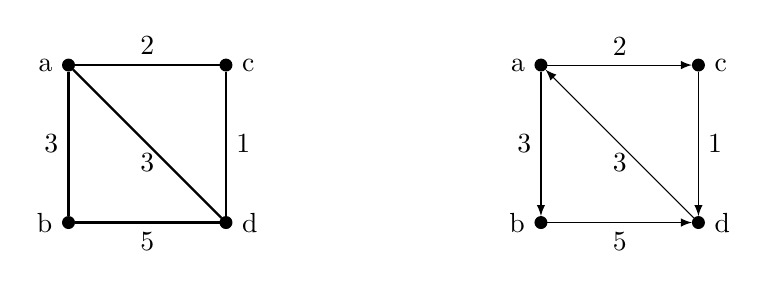
\begin{tikzpicture}
      \tikzset{enclosed/.style={draw, circle, inner sep=0pt, minimum size=.15cm, fill=black}}
%% Vertices
	%ikke orienteret
      	\node[enclosed, label={left, above: a}] (a) at (0,2) {};
     	\node[enclosed, label={left, below: b}] (b) at (0,0) {};
     	\node[enclosed, label={right, above: c}] (c) at (2,2) {};
     	\node[enclosed, label={right, below: d}] (d) at (2,0) {};
	%orienterede
		\node[enclosed, label={left, above: a}] (a1) at (6,2) {};
     	\node[enclosed, label={left, below: b}] (b1) at (6,0) {};
     	\node[enclosed, label={right, above: c}] (c1) at (8,2) {};
     	\node[enclosed, label={right, below: d}] (d1) at (8,0) {};
%Edges
	%Ikke orientered
		\path [thick] (a) edge node[midway, left] {3} (b);
		\path [thick] (a) edge node[midway, above] {2} (c);
		\path [thick] (b) edge node[midway, below] {5} (d);
		\path [thick] (c) edge node[midway, right] {1} (d);
		\path [thick] (a) edge node[midway, below] {3} (d);
	%orienterede
		\path [->, > = latex] (a1) edge node[midway, left] {3} (b1);
		\path [->, > = latex] (a1) edge node[midway, above] {2} (c1);
		\path [->, > = latex] (b1) edge node[midway, below] {5} (d1);
		\path [->, > = latex] (c1) edge node[midway, right] {1} (d1);
		\path [->, > = latex] (d1) edge node[midway, below] {3} (a1);

	\end{tikzpicture}
	\caption{Eksempel på en ikke orienteret vægte graf (venstre) og en orienteret vægtet graf (højre)}
	\label{fig.vaegteteks}
\end{figure}